
\excercise{DemoTask und UI}

\begin{enumerate}
    \item Nun wollen wir wieder ein Spiel starten. Diesesmal mit einem Task:

    \begin{lstlisting}
Game myGame = new Game("Hello World", new DemoTask());
    \end{lstlisting}

    Nun wollen wir das Spiel (Game) auch starten können. Also führen wir die Operation .run() darauf aus.

    \begin{lstlisting}
myGame.run();
    \end{lstlisting}

    Starte das Spiel in Eclipse, mit dem kleinen Play-Button oben in der Werkzeugleiste und schau dich ein wenig im Fenster um das aufgeht.

    \item Nun erweitern wir den Konstruktor von \texttt{Game} um einen Parameter. Erweitere den den Konstruktor um ein TaskVerifier Objekt, so wie unten im Bild zu sehen. Starte nun das Spielfenster neu. Was verändert sich im Spielfenster? Finde den Task Status und drücke den Refresh Button.

    \begin{lstlisting}
Game myGame = new Game("Hello World", new DemoTask(),
                        new DemoTaskVerifier());
    \end{lstlisting}

    \end{enumerate}
    \begin{Infobox}[Der Refresh Button]
    Wenn ihr überprüfen wollt ob ihr eure Aufgabe erledigt habt, müsst ihr auf \fbox{Task Status} und dann auf \fbox{Refresh} klicken.
    Wichtig: Der Task Status aktualisiert sich nicht automatisch.
    \end{Infobox}
    \begin{enumerate}\setcounter{enumi}{2}

    \item Finde sowohl im Spiel als auch in Eclipse die Konsole. Dies ist ein Feld in dem Text ausgegeben wird:
    \begin{center}
        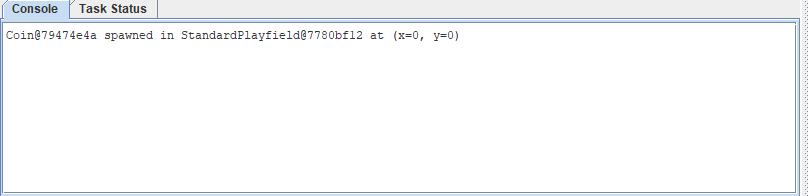
\includegraphics[width=\linewidth]{./figures/console.PNG}
    \end{center}

    In der Konsole siehst du, das eine Münze (\texttt{Coin}) gespawnt wurde. Finde die Koordinaten des Feldes, auf welchem die Münze gespawnt wurde.

    \item Nun suche nach der Stelle im Code in dem die erste Münze erzeugt wird. Kleiner Tipp: Verwende dafür  entweder \fbox{Strg} um auf Objekte zu klicken und in ihre Klasse zu kommen oder den PackageExplorer um in das Paket \texttt{de.unistuttagrt.informatik.fius.jvk.tasks} zu navigieren.
\end{enumerate}
